\documentclass[aspectratio=169]{beamer}

\usepackage[utf8]{inputenc}
\usepackage{beamerthemesplit}
\usepackage[orientation=landscape,size=custom,width=16,height=9,scale=0.5,debug]{beamerposter} 
\usepackage{graphicx}
\usetheme{Madrid}
\definecolor{UBCblue}{rgb}{0.04706, 0.13725, 0.26667}
\usecolortheme[named=UBCblue]{structure}

\titlegraphic{\vspace*{-1.7cm}
\includegraphics[width=2.8cm]{pictures/logo_cvut.png}\hspace*{10cm}~%

\includegraphics[width=2.1cm]{pictures/Grass_GIS_logo.png}
}

\AtBeginSection[]{
  \begin{frame}
  \vfill
  \centering
  \begin{beamercolorbox}[sep=8pt,center,shadow=true,rounded=true]{title}
    \usebeamerfont{title}\insertsectionhead\par%
  \end{beamercolorbox}
  \vfill
  \end{frame}
}

%Information to be included in the title page:
\title[Creation of a new GRASS GIS startup mechanism] %optional
{Creation of a new GRASS GIS startup mechanism}

\author[Bc. Linda Kladivova] % (optional, for multiple authors)
{Bc. Linda Kladivova}

\institute[Department of Geomatics] % (optional)
{
  CTU in Prague\\
  Faculty of Civil Engineering\\
  Department of Geomatics\\
  [8ex]
{\small Supervisor: Ing. Martin Landa, Ph.D.}
}

\date[February 4, 2021] % (optional)
{February 4, 2021}

\begin{document}

\frame{\titlepage}

\begin{frame}
\frametitle{Table of Contents}
\tableofcontents
\end{frame}

% Startovací mechanismus ve verzi 7.8
\section{Startup mechanism in the version 7.8}
\begin{frame}
\frametitle{Startup screen and data hierarchy}
\begin{itemize}
\item	Every GRASS GIS user was always redirected to the Startup screen
\item	Quite confusing without knowing what each of data hiearchy elements means
\end{itemize}
		\centering
	        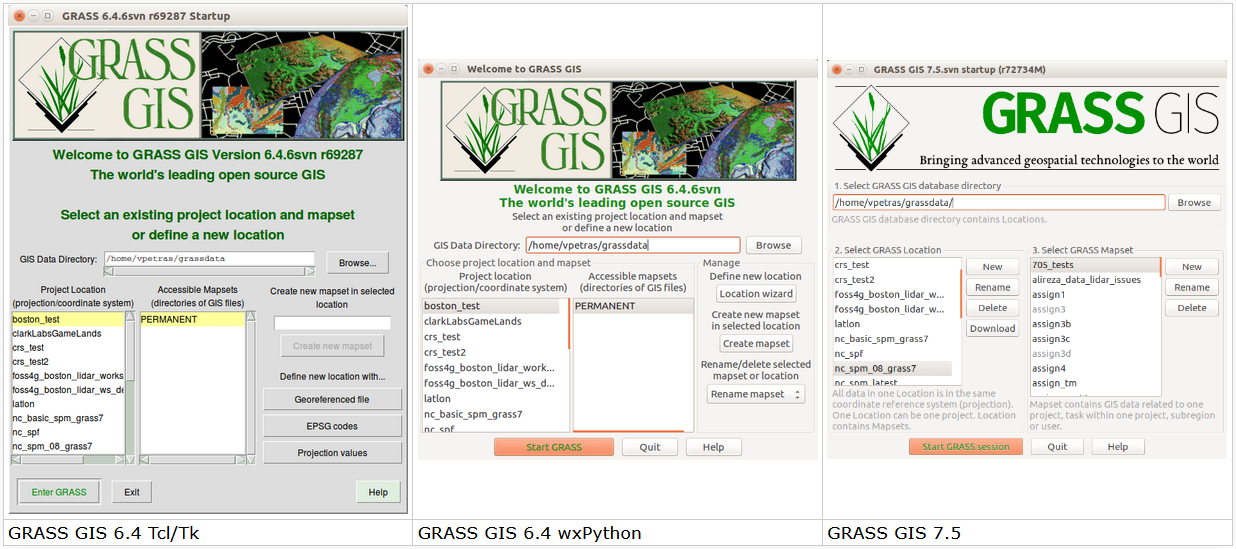
\includegraphics[width=0.8\columnwidth]{pictures/verze_startup.png}
\end{frame}

\begin{frame}
\frametitle{User complaints}
	        	\centering
	        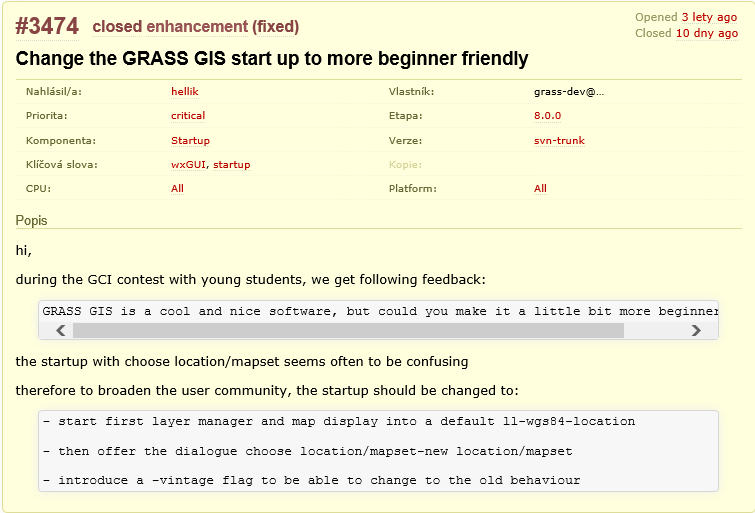
\includegraphics[width=0.8\columnwidth]{pictures/ticket.PNG}
\end{frame}

% Startovací mechanismus po GSoC
\section{Startup mechanism after GSoC}

\begin{frame}
\frametitle{Google Summer of Code}
	\centering
        
\includegraphics[width=0.7\textwidth]{pictures/Certificate.pdf}
\end{frame}

\begin{frame}
\frametitle{No more Startup screen for first-time user}
\begin{itemize}
\item Launched directly in the Data Catalog with the prepared \textit{default location (demolocation)} including world map in EPSG:4326
\end{itemize}
	\centering
        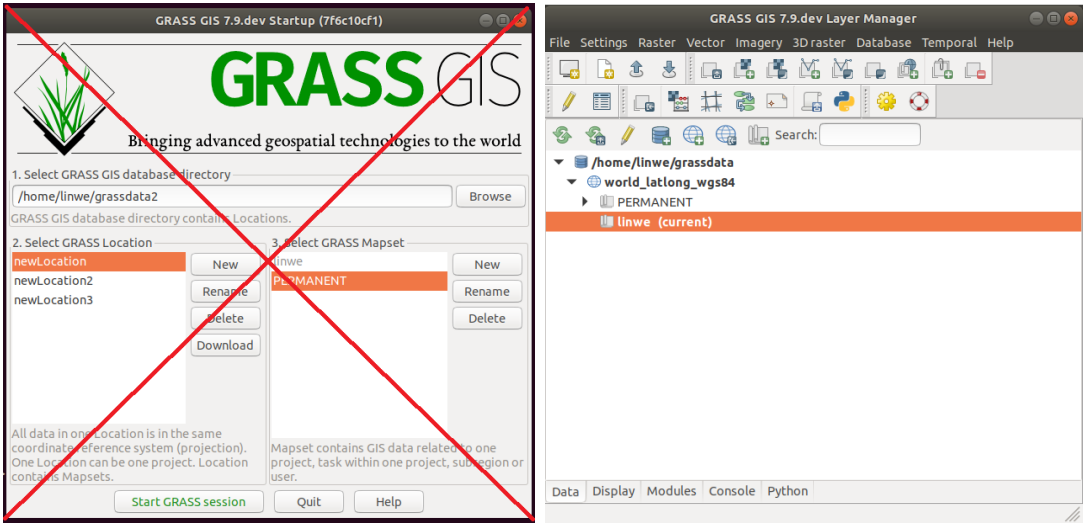
\includegraphics[width=0.8\textwidth]{pictures/demolocation_startup.PNG}
\end{frame}

\begin{frame}
\frametitle{No more Startup screen when start in the last used mapset}
\begin{itemize}
\item Launched directly in the Data Catalog
\item Used GRASS databases that had been stored in settings
\end{itemize}
	\centering
        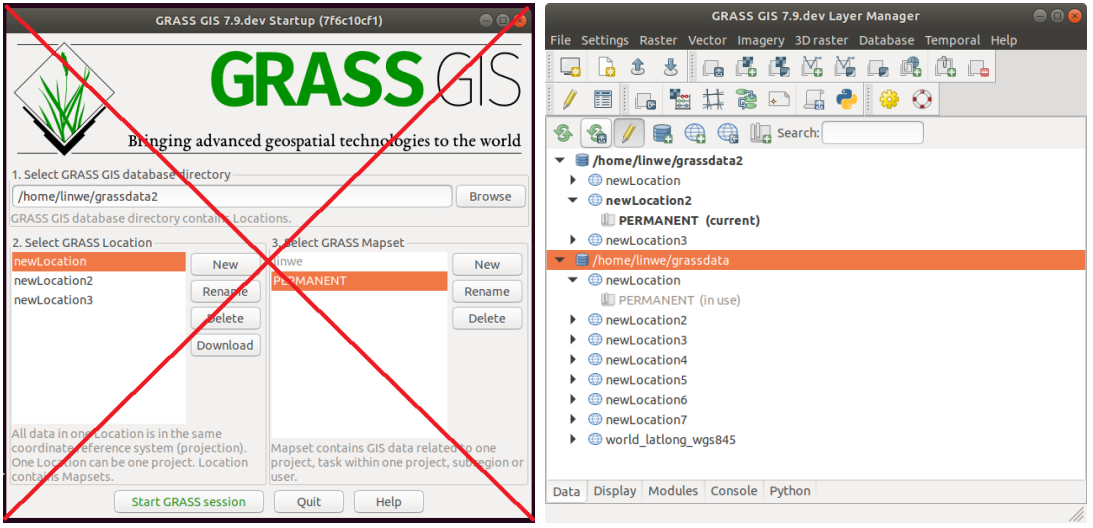
\includegraphics[width=0.8\textwidth]{pictures/last_mapset_startup.png}
\end{frame}

\begin{frame}
\frametitle{New functionalities in Data Catalog}
\begin{itemize}
\item Data Catalog takes over the role of startup screen and offers even more!
\end{itemize}
	\centering
        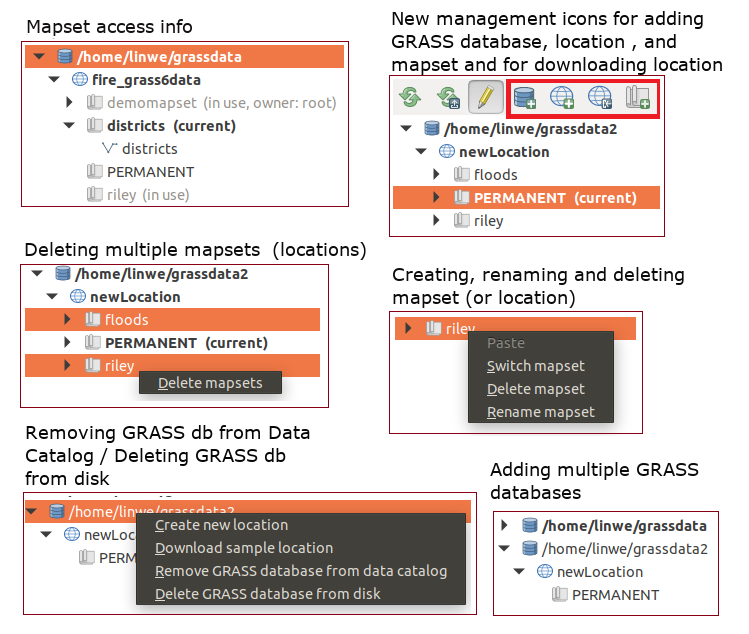
\includegraphics[width=0.5\textwidth]{pictures/funkce.PNG}
\end{frame}

\begin{frame}
\frametitle{For comparison - Poor Data Catalog before GSoC}
	        	\centering
	        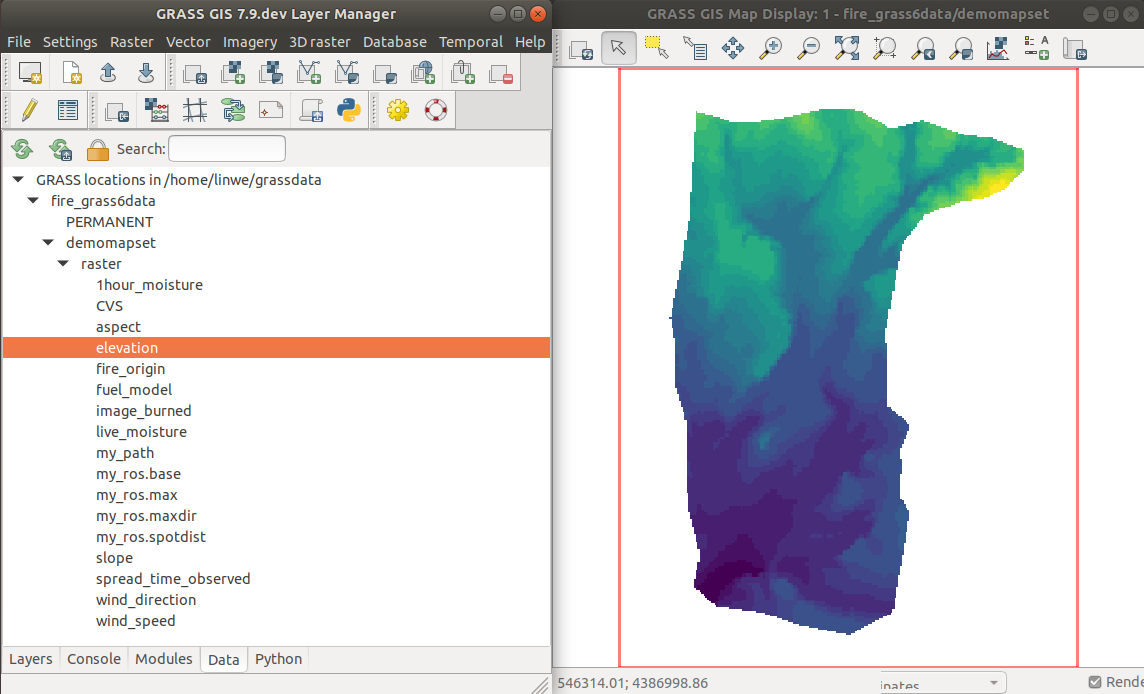
\includegraphics[width=0.8\columnwidth]{pictures/data_catalog_pred.PNG}
\end{frame}

\begin{frame}
\frametitle{Lacks of the solution after GSoC}
\begin{itemize}
\item Missing advice about how the first-time user should continue in data processing when he is in the default location
\vspace{0.5cm}
\item Old startup screen is still used when the last used mapset is not available (deleted or used by another user)
\end{itemize}
\end{frame}


\section{Thesis objectives}

\begin{frame}
\frametitle{Aims of the work}
\begin{itemize}
\item Evaluate the changes made during GSoC
\vspace{1cm}
\item Propose the solution for the new startup mechanism
\vspace{1cm}
\item Propose and implement a special mode for first-time users
\end{itemize}
\end{frame}


\section{Evaluate the changes made during GSoC}

\begin{frame}
\frametitle{Survey 1 Part 1: Help improve GRASS GIS startup mechanism and Data Catalog}
General questions:
\begin{itemize}
\item Are users satisfied with the new solution after GSoC?
\item Which new functionalities do they like the most?
\item What are general user preferences regarding further development of GRASS GUI?
\vspace{0.5cm}
\item Survey 1 Part 1 attended by 52 GRASS GIS users (all levels of proficiency)
\end{itemize}
\end{frame}


\begin{frame}
\frametitle{Evaluation of changes made during GSoC}

\begin{itemize}
\item Most of respondents like the situation after GSoC, however, there is also a minority of negative opinions.
\vspace{0.5cm}
\item Users appreciate the new Data Catalog management icons,  new small icons distinguishing mapsets, locations, GRASS
databases and layers (vector, raster) and new context menu options to create, rename and delete a mapset or location.
\vspace{0.5cm}
\item Users rate surprisingly low the new option of adding more GRASS databases (working directories).
\end{itemize}
\end{frame}

\section{Propose the solution for the new startup mechanism}

\begin{frame}
\frametitle{Survey 1 Part 1: Help improve GRASS GIS startup mechanism and Data Catalog}
Lack:
\begin{itemize}
\item  Old startup screen is still used when the last used mapset is not available (deleted or used by another user)
\end{itemize}

\vspace{0.5cm}
General question:
\begin{itemize}
\item How to improve the GRASS GIS startup mechanism?
\end{itemize}
\end{frame}

\begin{frame}
\frametitle{Propose the solution for the new startup mechanism}
\begin{itemize}
\item The author introduced two proposals
\vspace{0.5cm}
\item both permanently remove the old startup screen
\vspace{0.5cm}
\item both inspired by Infobar solution for first-time user mode
\end{itemize}
\end{frame}

\begin{frame}
\frametitle{GRASS GIS startup mechanism - Proposal 1}
\begin{columns}
\begin{column}{.35\textwidth}
\begin{itemize}
\item If the last mapset is not in the usable state GRASS starts into PERMANENT mapset in the default location with explaining infobar
\end{itemize}
\end{column}
\begin{column}{.65\textwidth}
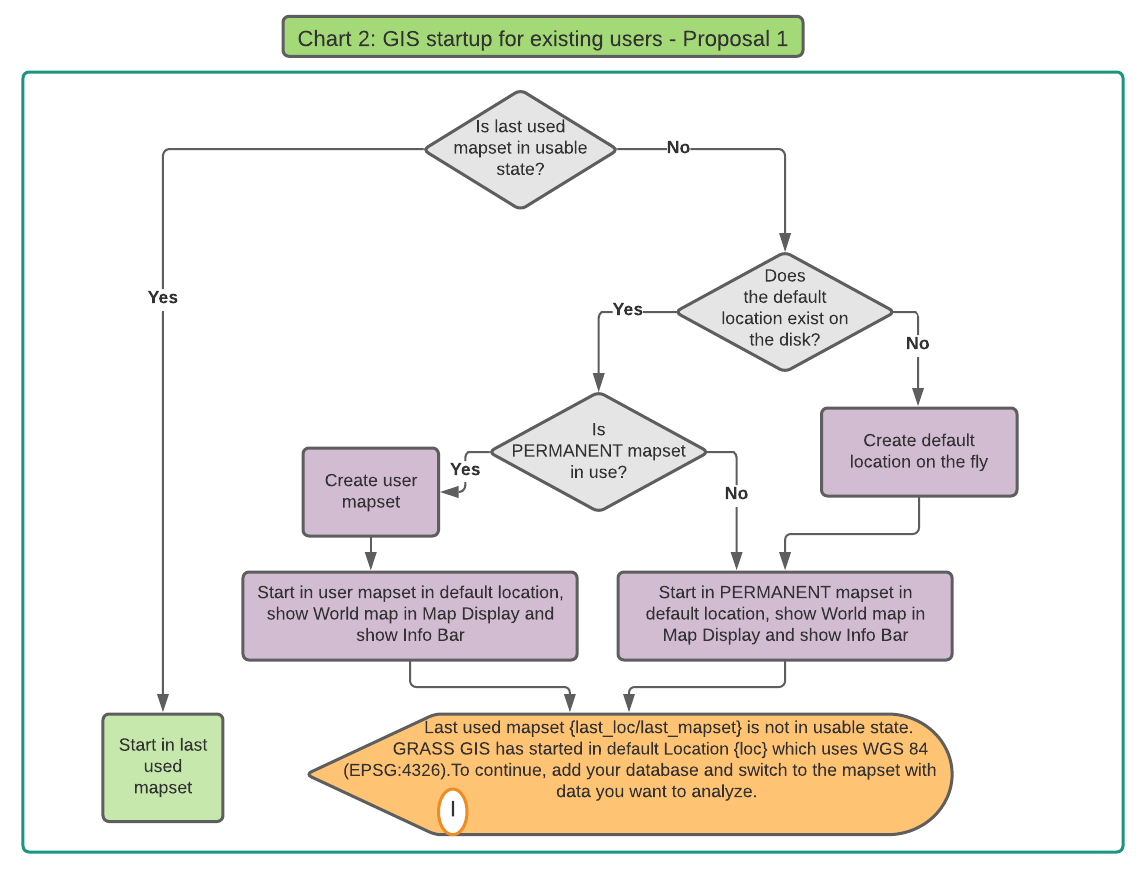
\includegraphics[width=\textwidth]{pictures/normal_user_diagram.PNG} \hspace*{4cm}
\end{column}
\end{columns}
\end{frame} 

\begin{frame}
\frametitle{GRASS GIS startup mechanism - Proposal 2}
\begin{columns}
\begin{column}{.35\textwidth}
\begin{itemize}
\item GRASS starts into PERMANENT mapset of last used location if possible, otherwise into PERMANENT mapset in the default location as in Proposal 1
\end{itemize}
\end{column}
\begin{column}{.65\textwidth}
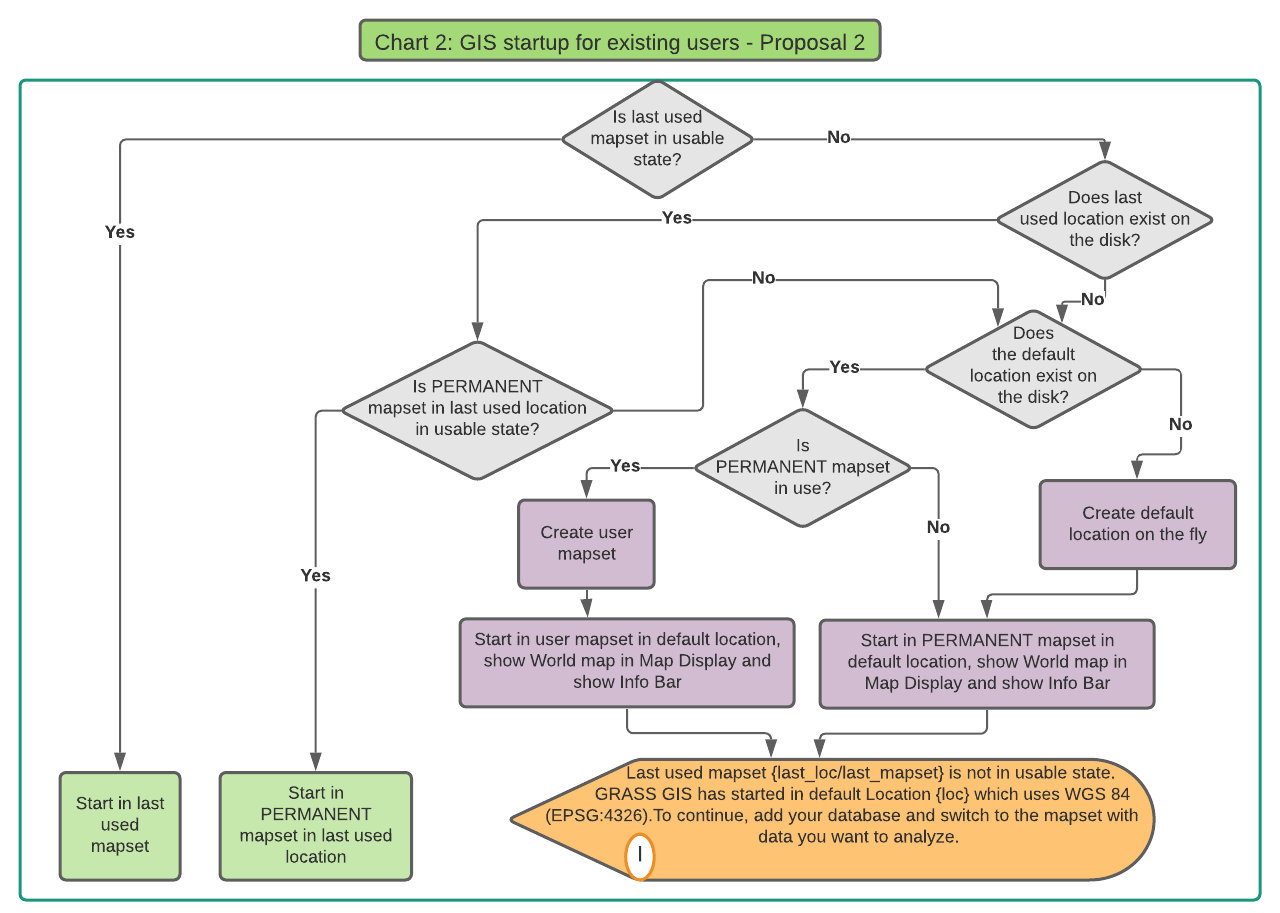
\includegraphics[width=\textwidth]{pictures/normal_user_diagram2.PNG} \hspace*{4cm}
\end{column}
\end{columns}
\end{frame} 

\section{Propose and implement a special mode for first-time users}

\begin{frame}
\frametitle{Survey 1 Part 2: Help create a better first-time user experience in GRASS GIS}
Lack:
\begin{itemize}
\item Missing advice about how the first-time user should continue in data processing when he is in the default location
\end{itemize}

\vspace{0.5cm}
General questions:
\begin{itemize}
\item What information the special mode for first-time users should contain?
\item Which implementation form to choose?
\vspace{0.5cm}
\item Survey 1 Part 2 attended by 48 GRASS GIS users (all levels of proficiency)
\end{itemize}
\end{frame}

\begin{frame}
\frametitle{Three key problematic first-time user situations identified on the basis of Survey 1 Part 2}

\begin{itemize}
\item{\textbf{Situation 1}: immediately after startup - a user needs to at least passively understand the principle of GRASS data hiearchy in order to create new Location with CRS of his data.}
\vspace{0.5cm}
\item{\textbf{Situation 2}: once a user creates a new location he needs to know how to import his data.}
\vspace{0.5cm}
\item{\textbf{Situation 3}: after importing the data, a user wants to either analyze data directly or change its display in the Map Display. So, he needs to know Display and Modules tabs.}
\end{itemize}
\end{frame}

\begin{frame}
\frametitle{Example of proposed infobar for first-time user after Survey 1}
	\centering
        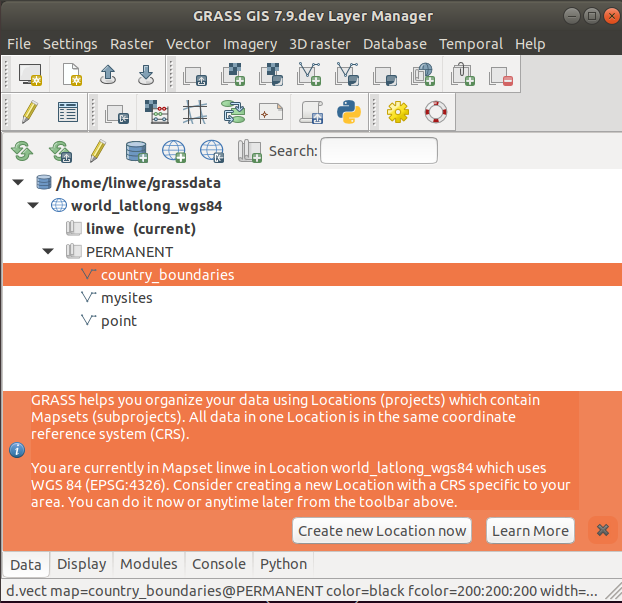
\includegraphics[width=0.55\textwidth]{pictures/info1before.PNG}
\end{frame}

\begin{frame}
\frametitle{Survey 2: Help improve the special mode for first-time users}
General questions:
\begin{itemize}
\item Do users like the proposed infobar?
\item Do they have any other ideas so that the implemented solution is the best from an objective point of view?
\vspace{0.4cm}
\item Survey 2 attended by 15 frequent GRASS users and 10 occasional GRASS users
\end{itemize}
\end{frame}

\begin{frame}
\frametitle{Impact of Survey 2 on the work}
	\centering
        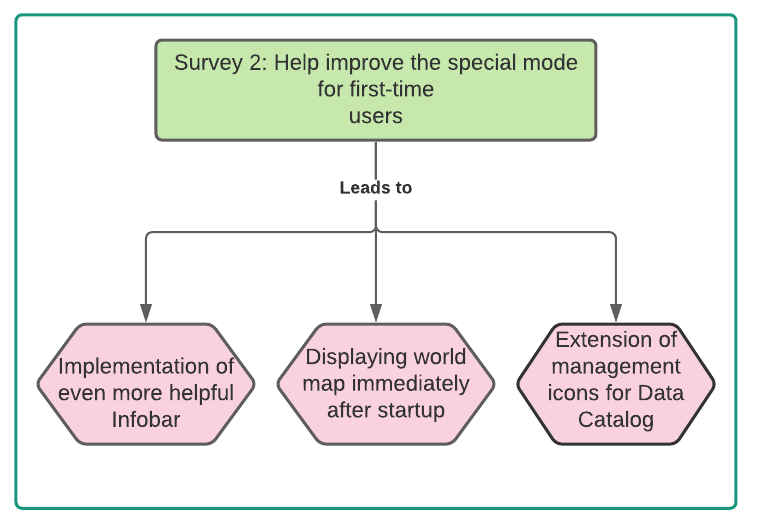
\includegraphics[width=0.7\textwidth]{pictures/survey2.PNG}
\end{frame}

\begin{frame}
\frametitle{Situation 1 before and after Survey 2, User mapset removed}
	\centering
        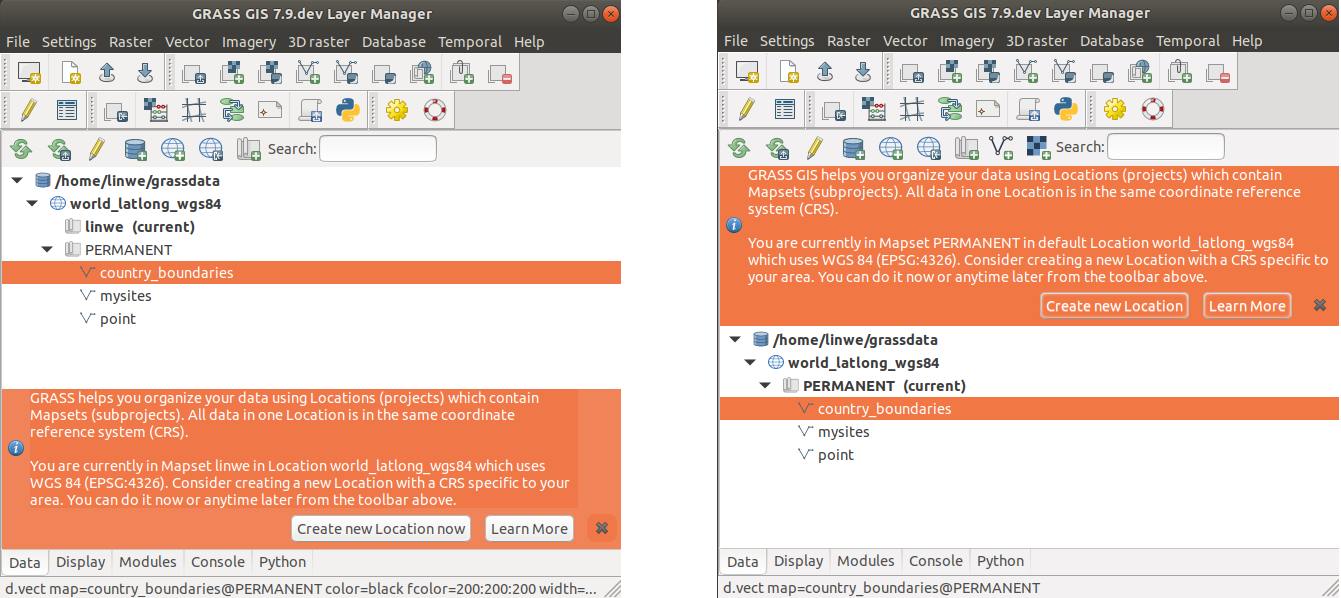
\includegraphics[width=0.95\textwidth]{pictures/info1.PNG}
\end{frame}

\begin{frame}
\frametitle{Situation 2 before and after Survey 2, New management icons for data import}
	\centering
        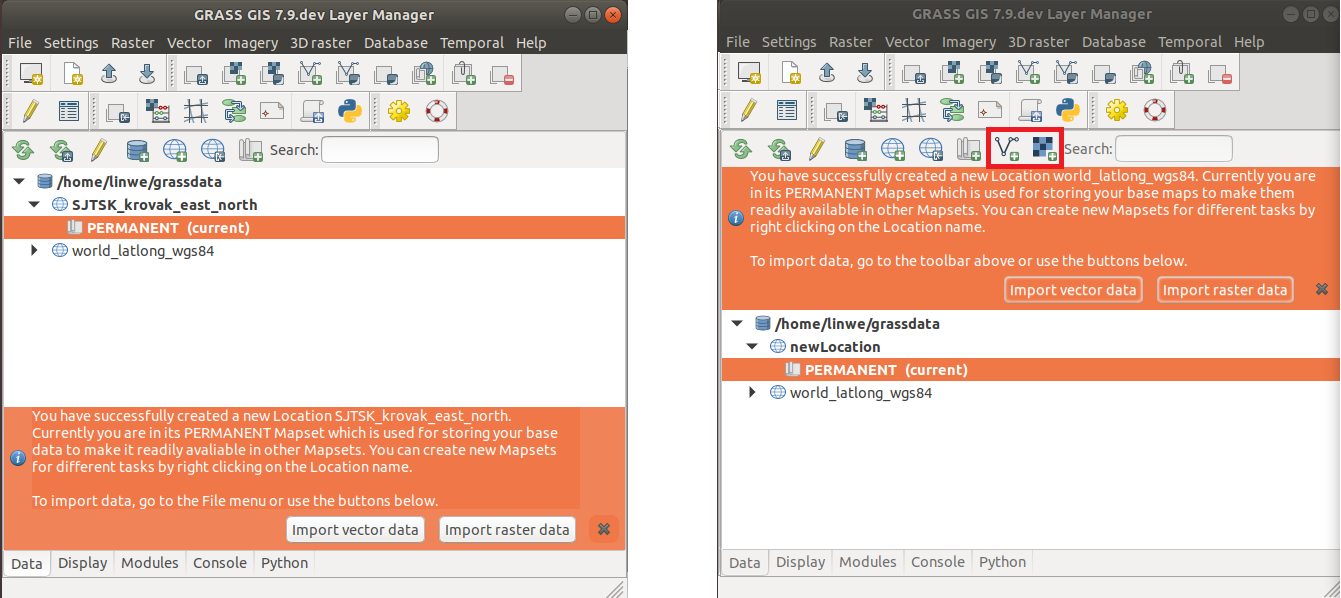
\includegraphics[width=0.95\textwidth]{pictures/info2.PNG}
\end{frame}

\begin{frame}
\frametitle{Situation 3 before and after Survey 2}
	\centering
        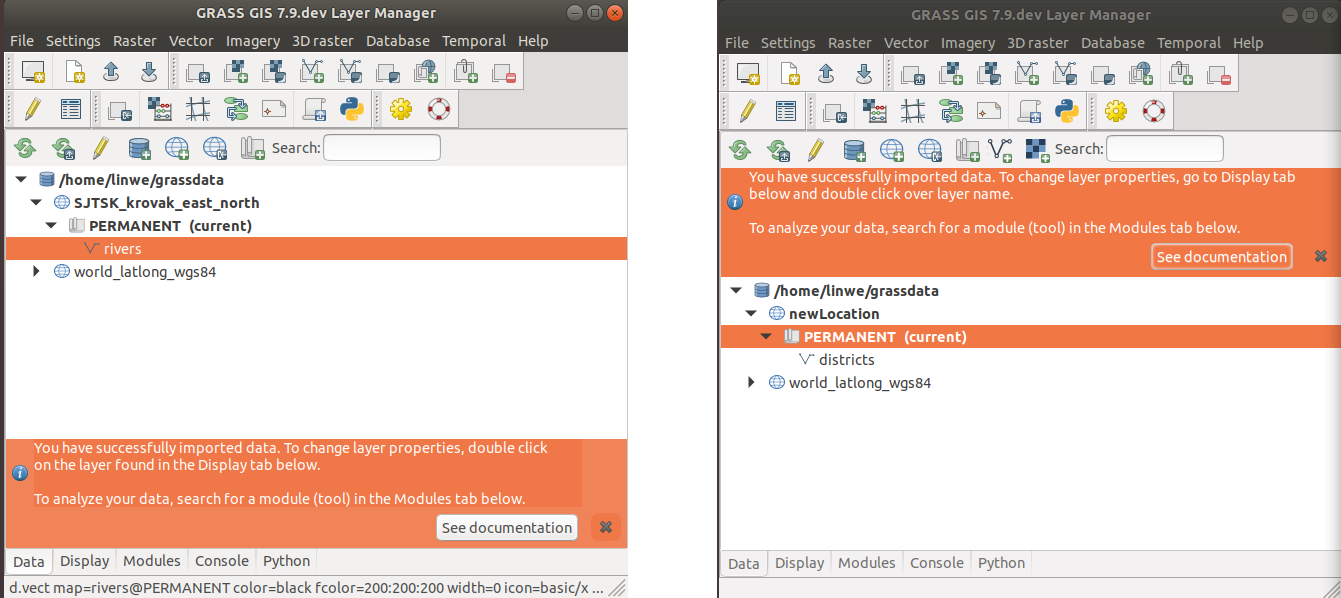
\includegraphics[width=0.95\textwidth]{pictures/info3.PNG}
\end{frame}

\begin{frame}
\frametitle{Displaying world map immediately after startup}
	\centering
        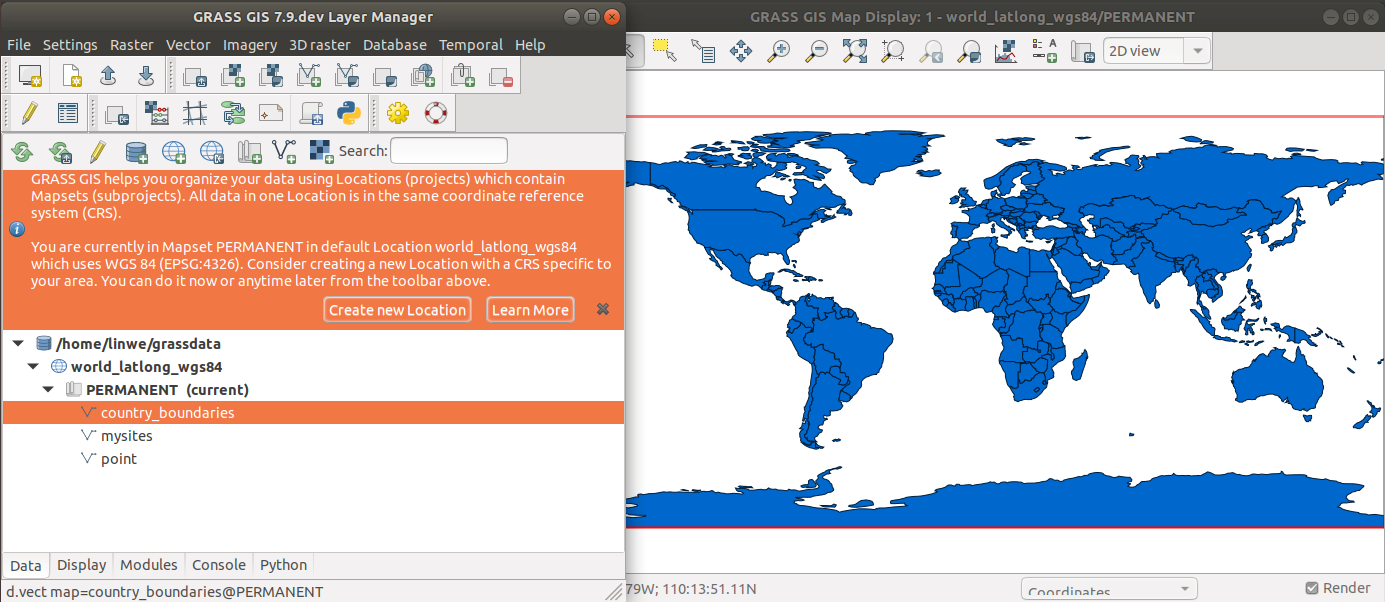
\includegraphics[width=0.95\textwidth]{pictures/po_prvnich_trech_PRs.PNG}
\end{frame}

\section{Conclusions}

\begin{frame}
\frametitle{Conclusions}
\begin{itemize}
\item{Most users like the partial removal of startup screen and improvements of the Data Catalog made during GSoC}
\vspace{0.5cm}
\item{Proposals for GRASS GIS startup machanism for normal users were introduced to GRASS community and they are now being discussed}
\vspace{0.5cm}
\item{GSoC improvements and the special mode for first-time users are already in the development GRASS branch}
\vspace{0.5cm}
\item{They will be part of the stable version 8.0 scheduled for the spring of 2021}
\end{itemize}
\end{frame}

\begin{frame}
\begin{center}
{\fontsize{20}{40}\selectfont Thank you for your attention}
\end{center}
\end{frame}

\section{Questions}

\begin{frame}
\frametitle{Supervisor's Question}
\begin{enumerate}
\item{Většina vámi navržených úprav byla začleněna do zdrojových kódů systému GRASS. Definitivní odstranění tradiční startovací obrazovky není nadšeně přijato všemi uživateli. Jak byste řešila snahu minimalizovat negativní ohlasy, které s sebou tento krok přináší?}
\end{enumerate}
\begin{itemize}
\vspace{0.3cm}
\item{V průzkumu 70 \% uživatelů pro začlenění modernizované startup screen, 30 \% pro využití defaultní lokace}
\item{Hlavní důvodem pravděpodobně nedostatečné pochopení komunity, že Data Catalog převzal a dokonce rozšířil roli startovací obrazovky}
\item{Založena nová diskuze na GitHub platformě -- podrobné vysvětlení a dialog ohledně obou představených návrhů}

\end{itemize}
\end{frame}

\begin{frame}
\frametitle{Opponent's Question 1}
\begin{enumerate}
\item{You used a definition of usability as ``to whether or not users can achieve specific goals with efficiency, effectinevess, and satisfaction''. How would that definition translate to the GRASS GIS startup? What would characterize a most user-friendly startup mechanism?}
\end{enumerate}
\begin{itemize}
\vspace{0.3cm}
\item{The user is happy when GRASS GIS starts fast, without complicated dialogs and with right settings immediatelly enabling the user to start working.}
\vspace{0.3cm}
\item{Efficiency (efektivnost) -- complete the task fast}
\item{Effectiveness (účinnost) -- accompish a purpose and produce the intended result}
\item{Satisfaction (spokojenost) - the user is happy with the result}
\end{itemize}
\end{frame}

\begin{frame}
\frametitle{Opponent's Question 1}
\begin{enumerate}
\item{You used a definition of usability as ``to whether or not users can achieve specific goals with efficiency, effectinevess, and satisfaction''. How would that definition translate to the GRASS GIS startup? What would characterize a most user-friendly startup mechanism?}
\end{enumerate}
\begin{itemize}
\vspace{0.3cm}
\item{A good user-friendly startup mechanism}
\begin{itemize}
\item{opens the program}
\item{opens it fast}
\item{remembers the user's settings (in GRASS - start in the last used mapset)}
\item{can solve arisen problems (when last mapset not avaliable (deleted, in use or broken))}
\item{leads new users}
\item{creates no burden for professionals}
\end{itemize}
\end{itemize}
\end{frame}

\begin{frame}
\frametitle{Opponent's Question 2}
\begin{enumerate}\addtocounter{enumi}{1}
\item{What would be the five main topics on a long term roadmap for further UX development in GRASS GIS and why (consider effect and probably effort)?}
\end{enumerate}
\begin{itemize}
\vspace{0.3cm}
\item{Complete the issue of the startup mechanism} - medium effect, no consensus
\item{Strictly semantically separate Data and Display tabs} - big effect, medium effort
\item{Design GRASS GUI as a single window application} - huge effect as well as effort
\item{Make the Location Wizard more pleasant} - probably big effect as well as effort
\item{Enrich the Data Catalog functionalities beyond changes made during GSoC} - small effect as well as effort, but depends on functionalities
\end{itemize}
\end{frame}

\begin{frame}
\frametitle{Opponent's Questions 3}
\begin{enumerate}\addtocounter{enumi}{2}
\item{How does the concept of the PERMANENT mapset affect user experience? Is it an asset, irrelevant or an obstacle to new users?}
\end{enumerate}
\begin{itemize}
\vspace{0.3cm}
\item{PERMANENT mapset - automatically created, visible from other mapsets, used for storing data common to all projects}
\item{For experienced users (and multiple users accessing the same location) asset, for new users rather confusing}
\item{Effort to bring the PERMANENT mapset closer to new users by explaining it in the \textit{second infobar}}
\end{itemize}
\end{frame}

\begin{frame}
\frametitle{Opponent's Question 4}
\begin{enumerate}\addtocounter{enumi}{3}
\item{How does the search path concept integrate with the data catalog? Do you expect confusion among users when visible maps in the catalog are not available in modules interfaces?}
\end{enumerate}
\begin{itemize}
\vspace{0.3cm}
\item{Modules offer maps contained in PERMANENT or current mapset}
\item{Mapset Access Info was created to emphasize the function of the current mapset in the Data Catalog}
\item{Obvious that maps in another than the current mapset will not be offered to the user} 
\end{itemize}
\end{frame}


\end{document}
